\documentclass{beamer}

\usepackage{color}
\usepackage{ctex}
\usepackage{graphicx}
\usepackage{beamerthemesplit}
\usepackage{caption}
\usepackage{graphicx, subfig}


\title{Learning to Explain: An Information-Theoretic Perspective on Model Interpretation}
\author{Zhou Hao}
\date{2018.10}

\begin{document}
 	\frame{\titlepage}
 	\section*{Outline}
 	\frame{\tableofcontents}

 	\section{Introduction}
  \frame{
  \textbf{Introdunction} \\ 
  \begin{itemize}
    \item Why Model Interpretation?
    \item Instancewise feature selection
    \item What's different?
    \begin{itemize}
      \item propose an information-based framework for instancewise feature selection
      \item introduce a learning-based method for instancewise feature selection, which is both efficient and model-agnostic
    \end{itemize}
  \end{itemize}
  }

  \section{Framework}
  \frame{
  We assume one has access to the output of a model as a conditional distribution, $\mathbb{P}_m(\cdot \mid x)$, of the response variable Y given the realization of the input random variable $X = x \in \mathbb{R}^d$
  \begin{figure}
  \centering
  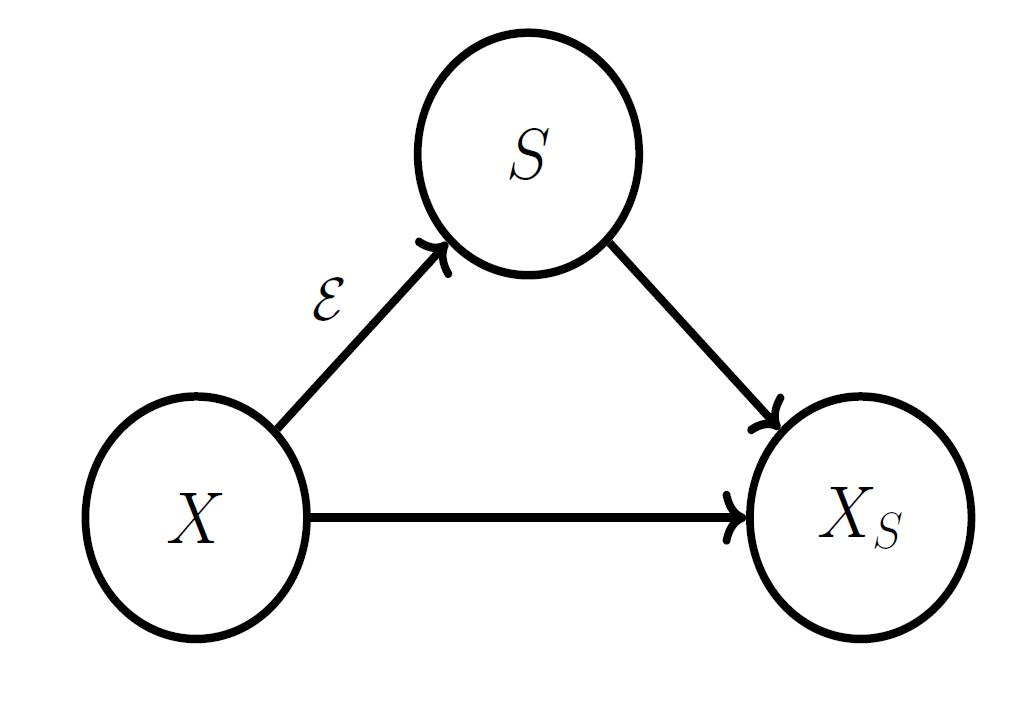
\includegraphics[width=.8\textwidth]{fig1.jpg}
  \end{figure}
  }
  
  \subsection{Mutual Information}
  \frame{
  \textbf{Mutual Information} \\
  $I(X;Y)$ is a measure of dependence between them, it corresponds to how much knowledge of random vector reduces the uncertainty about the other.

  $$I(X;Y) = \mathbb{E}_{X,Y}[\log \frac{p_{XY}(X,Y)}{p_X(X)p_Y(Y)}]$$
  }

  \subsection{How to construct explanations}
  \frame{
  \textbf{How to construct explanations}
  \begin{itemize}
      \item $\wp _{k} = \{S \subset 2^d | |S| = k\}$ is the set of all subsets of size $k$ \\
      \item An explainer $\varepsilon$ is a mapping from feature space $\mathbb{R}^d$ to the power set $\wp_k$ \\
      \item $X_S \in R^k$ is the sub-vector formed by the chosen features
      \item formulate instancewise feature selection as seeking explainer that optimizes the criterion 
      \begin{equation}
          \max_\varepsilon I(X_S;Y) \quad s.t. \quad S \sim \varepsilon(X)
      \end{equation}
  \end{itemize}
  }

  \section{Proposed method}
  \subsection{Obtaining a tractable variational formulation}
  \frame{
  \textbf{A variational lower bound}
  $$
  \begin{aligned}
    I(X_S;Y) &= E[\log \frac{P_m(X_S,Y)}{P(X_S)P(Y)}] = E[\log\frac{P_m(Y \mid X_S)}{P_m(Y)}] \\
             &= E[\log P_m(Y \mid X_S)] + Const \\
             &= E_X E_{S \mid X} E_{Y \mid X_S}[\log P_m(Y \mid X_S)] + Const \\
  \end{aligned}
  $$
  It's impossible to compute expectations under the conditional distribution
  }

  \frame{
  \begin{itemize}
      \item $$
  \begin{aligned}
    \mathcal{Q}  := \{\mathbb{Q} \mid \mathbb{Q}=\{X_S \rightarrow \mathbb{Q}_S(Y \mid X_S),S \in \wp_k\}\}
  \end{aligned}
  $$
  each $\mathbb{Q}$ is a collection of conditional distribution $\mathbb{Q}_S(Y \mid X_S)$, one for each choice of k-sized feature subset $S$
  \item $$\mathbb{E}_{Y \mid X_S}[\log \mathbb{P}_m(Y \mid X_S)] \geq \mathbb{E}_{Y \mid X_S}[\log \mathbb{Q}_S(Y \mid X_S)]$$
  problem can be relaxed as maximizing the variational lower bound, over both the explanation $\varepsilon$ and the conditional distribution $Q$:
  $$\max_{\varepsilon,\mathbb{Q}} \mathbb{E}[\log \mathbb{Q}_S(Y \mid X_S)] , S \sim \varepsilon(X)$$
  \end{itemize}
  }

  \frame{
  \textbf{A single neural network for parametrizing $\mathbb{Q}$} \\
  \begin{itemize}
    \item single neural network function:
  $$g_\alpha : \mathbb{R}^d \times [c] \rightarrow [0,1]$$
    \item We define:
  $$\mathbb{Q}_S(Y\mid x_S) := g_\alpha(\tilde{x}_S,Y)$$
  where $\tilde{x}_S$ is transformed from $x$
  \end{itemize}
  }

  \subsection{Continuous relaxation of subset sampling}
  \frame{
  \textbf{Continuous relaxation of subset sampling}\\
  \begin{itemize}
      \item random perturbation:
      $$G_i = -\log(-\log u_i), u_i \sim Uniform(0,1)$$
      \item temperature-dependent softmax:
      $$C_i = \frac{exp\{(\log p_i+G_i)/\tau\}}{\sum_{j=1}^d exp\{(\log p_i+G_i)/\tau\}}$$
      \item resulting random vector:
      $$C_i \sim Concrete(\log p_1,\cdots, \log p_d)$$
  \end{itemize}
  }

  \subsection{The final objective and its optimization}
  \frame{
  \textbf{The final objective and its optimization}\\
  \begin{itemize}
      \item after having applied the continuous approximation of feature subset sampling:
      $$\max_{\theta,\alpha}\mathbb{E}_{X,Y,\eta}[\log g_\alpha(V(\theta,\eta)\odot X,Y)]$$
      \item in the case of classification with $c$ classes:
      $$\mathbb{E}_{X,\eta}[\sum_{y=1}^c [\mathbb{P}_m(y \mid X) \log g_\alpha(V(\theta,\eta)\odot X,y)]$$
  \end{itemize}
  }

  \section{Experiment}
  \subsection{Efficiency}
  \frame{
  \textbf{Efficiency}
  \begin{figure}
  \centering
  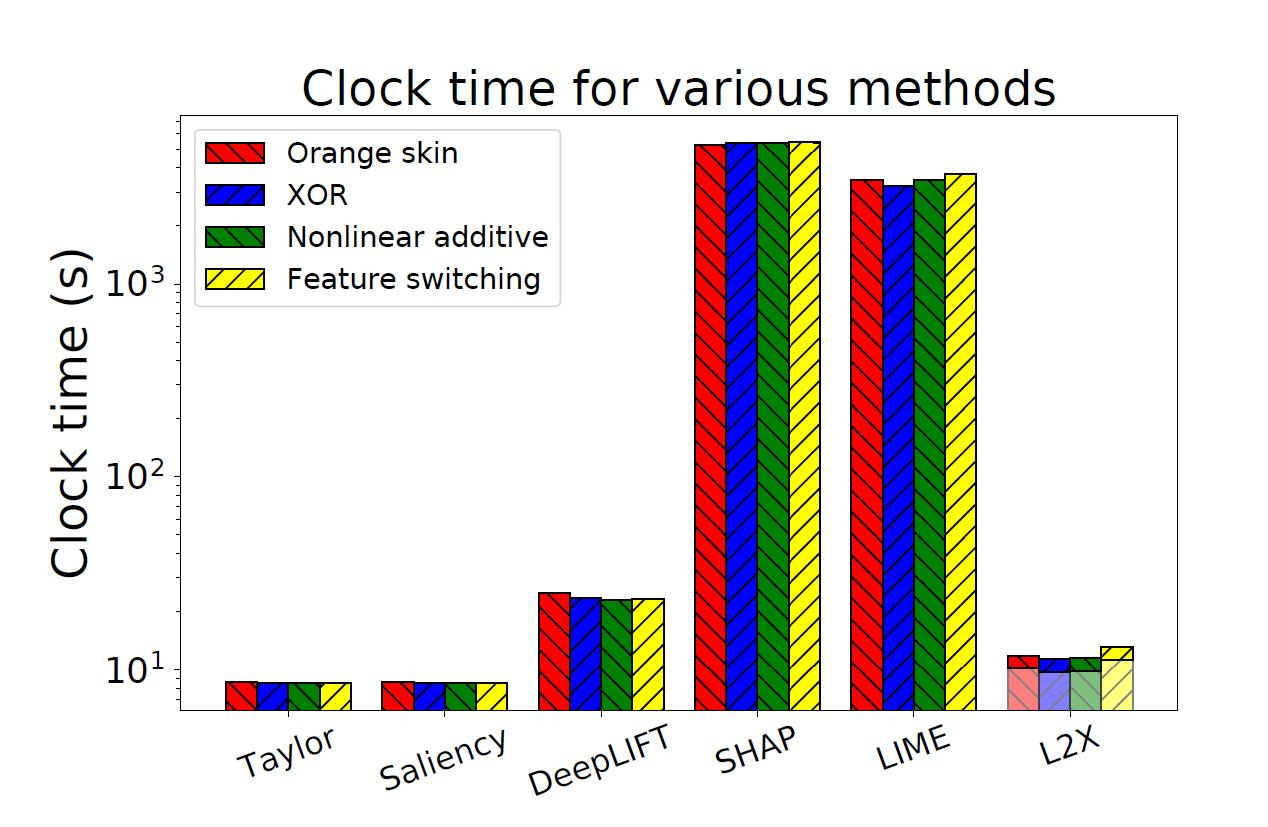
\includegraphics[width=.8\textwidth]{fig2.jpg}
  \end{figure}
  }
  
  \subsection{Accuracy}
  \frame{
  \textbf{Accuracy}
  \begin{itemize}
      \item Data:
      \begin{itemize}
          \item Synthetic Data
          \item IMDB
          \item MNIST
      \end{itemize}
      \item post-hoc accuracy \\
      We feed in the sample $X$ to the model with unselected words masked by zero paddings. Then we compute the accuracy of using $\mathbb{P}_m(y\mid \tilde{X}_S)$ to predict samples in the test data set
  \end{itemize}
  }
\end{document}
